\documentclass[letterpaper,11pt,oneside]{memoir}

\usepackage{xess}

\product[StickIt! Grove]
\manualnum{013}
\manualversion{1.0}
\newcommand{\copyrightyear}{2015}
\newcommand{\xula}{XuLA Board}
\newcommand{\stickit}{StickIt! Board}

\begin{document}

\frontmatter

\makexessmanualtitlepage{product_cover.jpg}{0.7}

\makexesslegal{\copyrightyear}

\begin{xessrevisiontbl}
	07/15/2015 & 1.0 & Initial release for \product\ V1.0.\\
%	\hline
%	06/04/2015 & 4.0 & Revised for \product\ V4.0.\\
\end{xessrevisiontbl}

\makexesstoc

\mainmatter



\chapter{Preliminaries}

Here's some helpful information before getting started.


\section{Getting Help!}

Here are some places to get help if you encounter problems:

\begin{itemize}
\item If you can't get the \product\ to work, send an e-mail message
	describing your problem to \href{mailto:\helpemail}{\helpemail}. 
\item Or submit a problem report at	\url{\helppage}.
\item \href{http://www.xess.com}{Our web site} also has
	\begin{itemize}
	\item \href{http://www.xess.com/projects/}{example designs}, 
	\item \href{http://www.xess.com/appnotes/}{application notes}, and
	\item \href{http://www.xess.com/tutorials/}{tutorials}.
%	\item answers to frequently-asked-questions,
%	\item \href{}{a forum where you can post questions}.
	\end{itemize}
\end{itemize}


% \section{Take Notice!}

% \begin{itemize}
% \item The \xula\ is not 5V-tolerant. \warning{Do not connect 5V logic signals
	% to the \digpmod\ sockets of the \product.}
% \item \warning{Only power the \product\ with a regulated 5 VDC,
	% center-positive power supply.}
% \end{itemize}


\section{Packing List}

Here is what you should have received in your package:

\begin{itemize}
	\item a \product.
	\item a 6\by 2 right-angle male header.
	\item two 5\by 1 male headers.
\end{itemize}



\chapter{Setup}

The \product\ provides sockets for connecting up to four Grove modules to
a single \digpmod\ socket on a \stickit, or it can be plugged into a solderless breadboard.

\section{Inserting Your \texorpdfstring{\product}{StickIt! Grove}\ Into Your \texorpdfstring{\stickit}{StickIt! Board}}

To use the \product\ with a \digpmod\ socket, first solder the 6\by 2 right-angle male header to the module.
Then the \product\ can be inserted into any of the \digpmod\ sockets of the \stickit\ as shown below.

\fixedpic{\includegraphics[width=0.7\textwidth]{pmod_insertion.jpg}}

\section{Inserting Your \texorpdfstring{\product}{StickIt! Grove}\ Into a Breadboard}

To use the \product\ with a solderless breadboard, first solder the two 5\by 1 male headers as shown.
Then the \product\ can be inserted into the breadboard as shown below.

\fixedpic{\includegraphics[width=0.7\textwidth]{breadboard_insertion.jpg}}



\chapter{Using the \product}

Each of the four Grove sockets receives two of the eight data lines that connect to the 
\digpmod\ and breadboard connectors.
Each Grove socket also shares a common ground and power connection with the \digpmod\ and
breadboard connectors.
Attaching a Grove module to one of the sockets provides the module with power, ground, and two I/O lines.


\section{Using the \product\ with a \stickit}

In order to interface a Grove module with a \stickit\ and \xula\ through a \digpmod\ socket, you have to figure out
the path the signals take from the pins of the FPGA through the \stickit\ and \digpmod\ sockets and finally on to the Grove module. 
You can manually trace the path using the following procedure:

\begin{itemize}
\item Connect the \product\ to one of the \digpmod\ sockets (PM1--PM3) on the \stickit.
\item \label{itm:groveconnect} Connect a Grove module to one of the sockets (GR1--GR4) on the \product\ and 
    note which \digpmod\ signals (D0--D7) it connects to.
\item Using the \digpmod\ socket and signal found in the previous steps, lookup
    the channel it connects to in the table on page 12 of the \href{http://www.xess.com/static/media/manuals/StickIt-manual-v4_0.pdf}{\stickit\ manual}.
\item Now use the channel to lookup the FPGA pin of the \xula\ it connects to in the
	table on page 9 of the \href{http://www.xess.com/static/media/manuals/StickIt-manual-v4_0.pdf}{\stickit\ manual}.
\item Make a UCF file associating each FPGA pin with each I/O of the module.
\item Include the UCF file in your Xilinx ISE FPGA project.
\end{itemize}

As an example, consider using a simple Grove module with a single LED.
Plugging the module into socket GR3 on the \product\ connects the LED's anode to pin D7 of the \digpmod\ connector
and its cathode to ground.
Inserting the \product\ into socket PM3 of the \stickit\ connects D7 to channel 30.
Assuming a XuLA2 board is inserted into the \stickit, channel 30 will terminate on
pin B2 of the FPGA.
So the UCF file would contain a constraint like this:

\begin{lstlisting}
net LED loc = B2;
\end{lstlisting}

Admittedly, that's a lot of work just to make a connection!
Instead of going through all that,
the |xsconnect| Python package (\url{https://pypi.python.org/pypi/xsconnect})
provides two scripts to make the process easier.
The command-line script generates the UCF directly like so:

\begin{lstlisting}
xsconn -p grove -m stickit4 -n pm3 -d xula2
\end{lstlisting}
    
which gives:

\begin{lstlisting}
########################################################################
# StickIt! Grove V1.0 ==[pm3]==> StickIt! V4 ==> XuLA2
net gr1-d0 loc = h2;
net gr1-d1 loc = f1;
net gr2-d2 loc = f2;
net gr2-d3 loc = e1;
net gr3-d6 loc = b1;
net gr3-d7 loc = b2;
net gr4-d4 loc = e2;
net gr4-d5 loc = c1;
########################################################################
\end{lstlisting}

The |gxsconn| script does the same thing, but with a GUI:

\fixedpic{\includegraphics[width=0.7\textwidth]{gxsconn.png}}

Just change the |gr3-d7| in the output to |LED| (or whatever name you want to use) and include
the constraint in the UCF file of your ISE project. 


\section{Using the \product\ with a Breadboard}

After inserting the \product\ into a breadboard, attaching a Grove module to one of the sockets
connects its two I/O signals to two of the pins D0--D7 connecting to the breadboard 
as well as the power and ground pins.
The pins associated with each Grove socket are printed next to each socket, and
the corresponding pin locations on the breadboard header are shown in the 
\hyperref[fig:connections]{figure on page~\pageref*{fig:connections}}.
Then just use jumpers or hookup wire to make connections from the header
to the rest of your circuitry on the breadboard.


\chapter{I/O Locations}

The connections of the \digpmod\ and breadboard I/O signals to the Grove sockets are shown below.

\fixedpic{\label{fig:connections}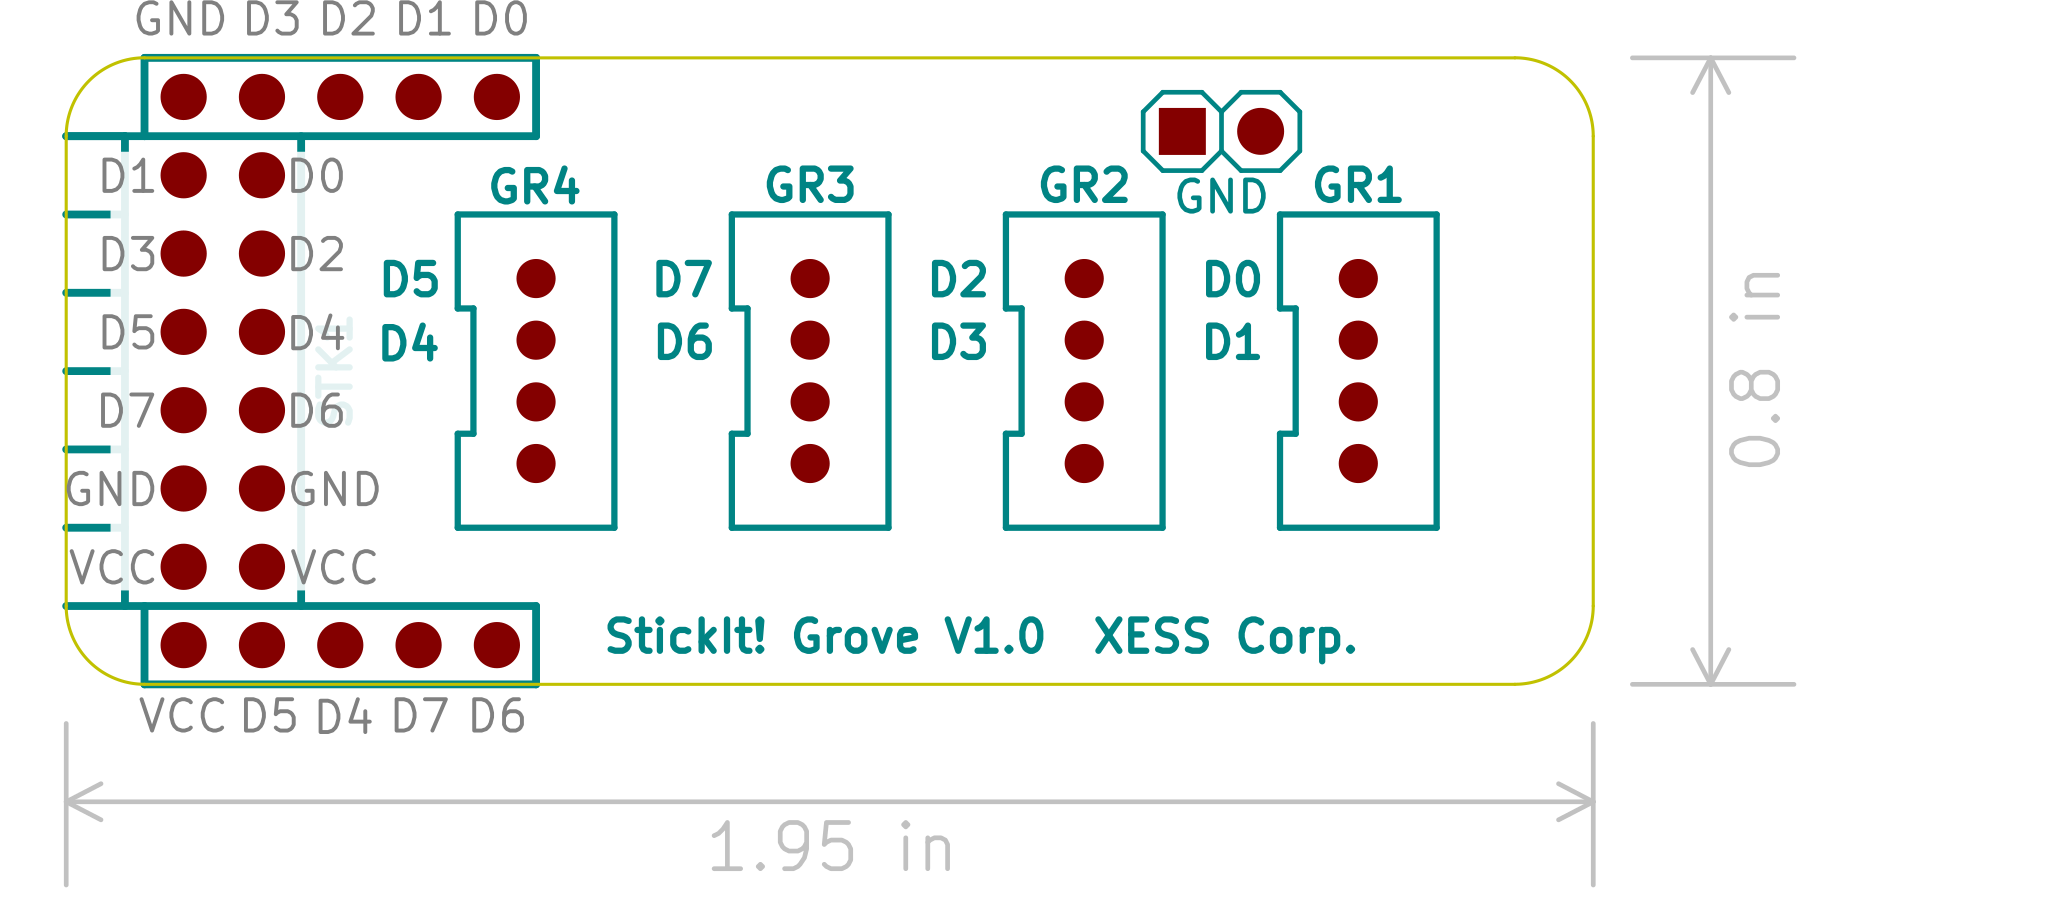
\includegraphics[width=0.7\textwidth]{grove_pcb.png}}

\chapter{Schematic}

\pagebreak
\makebox[\textwidth][r]{\hss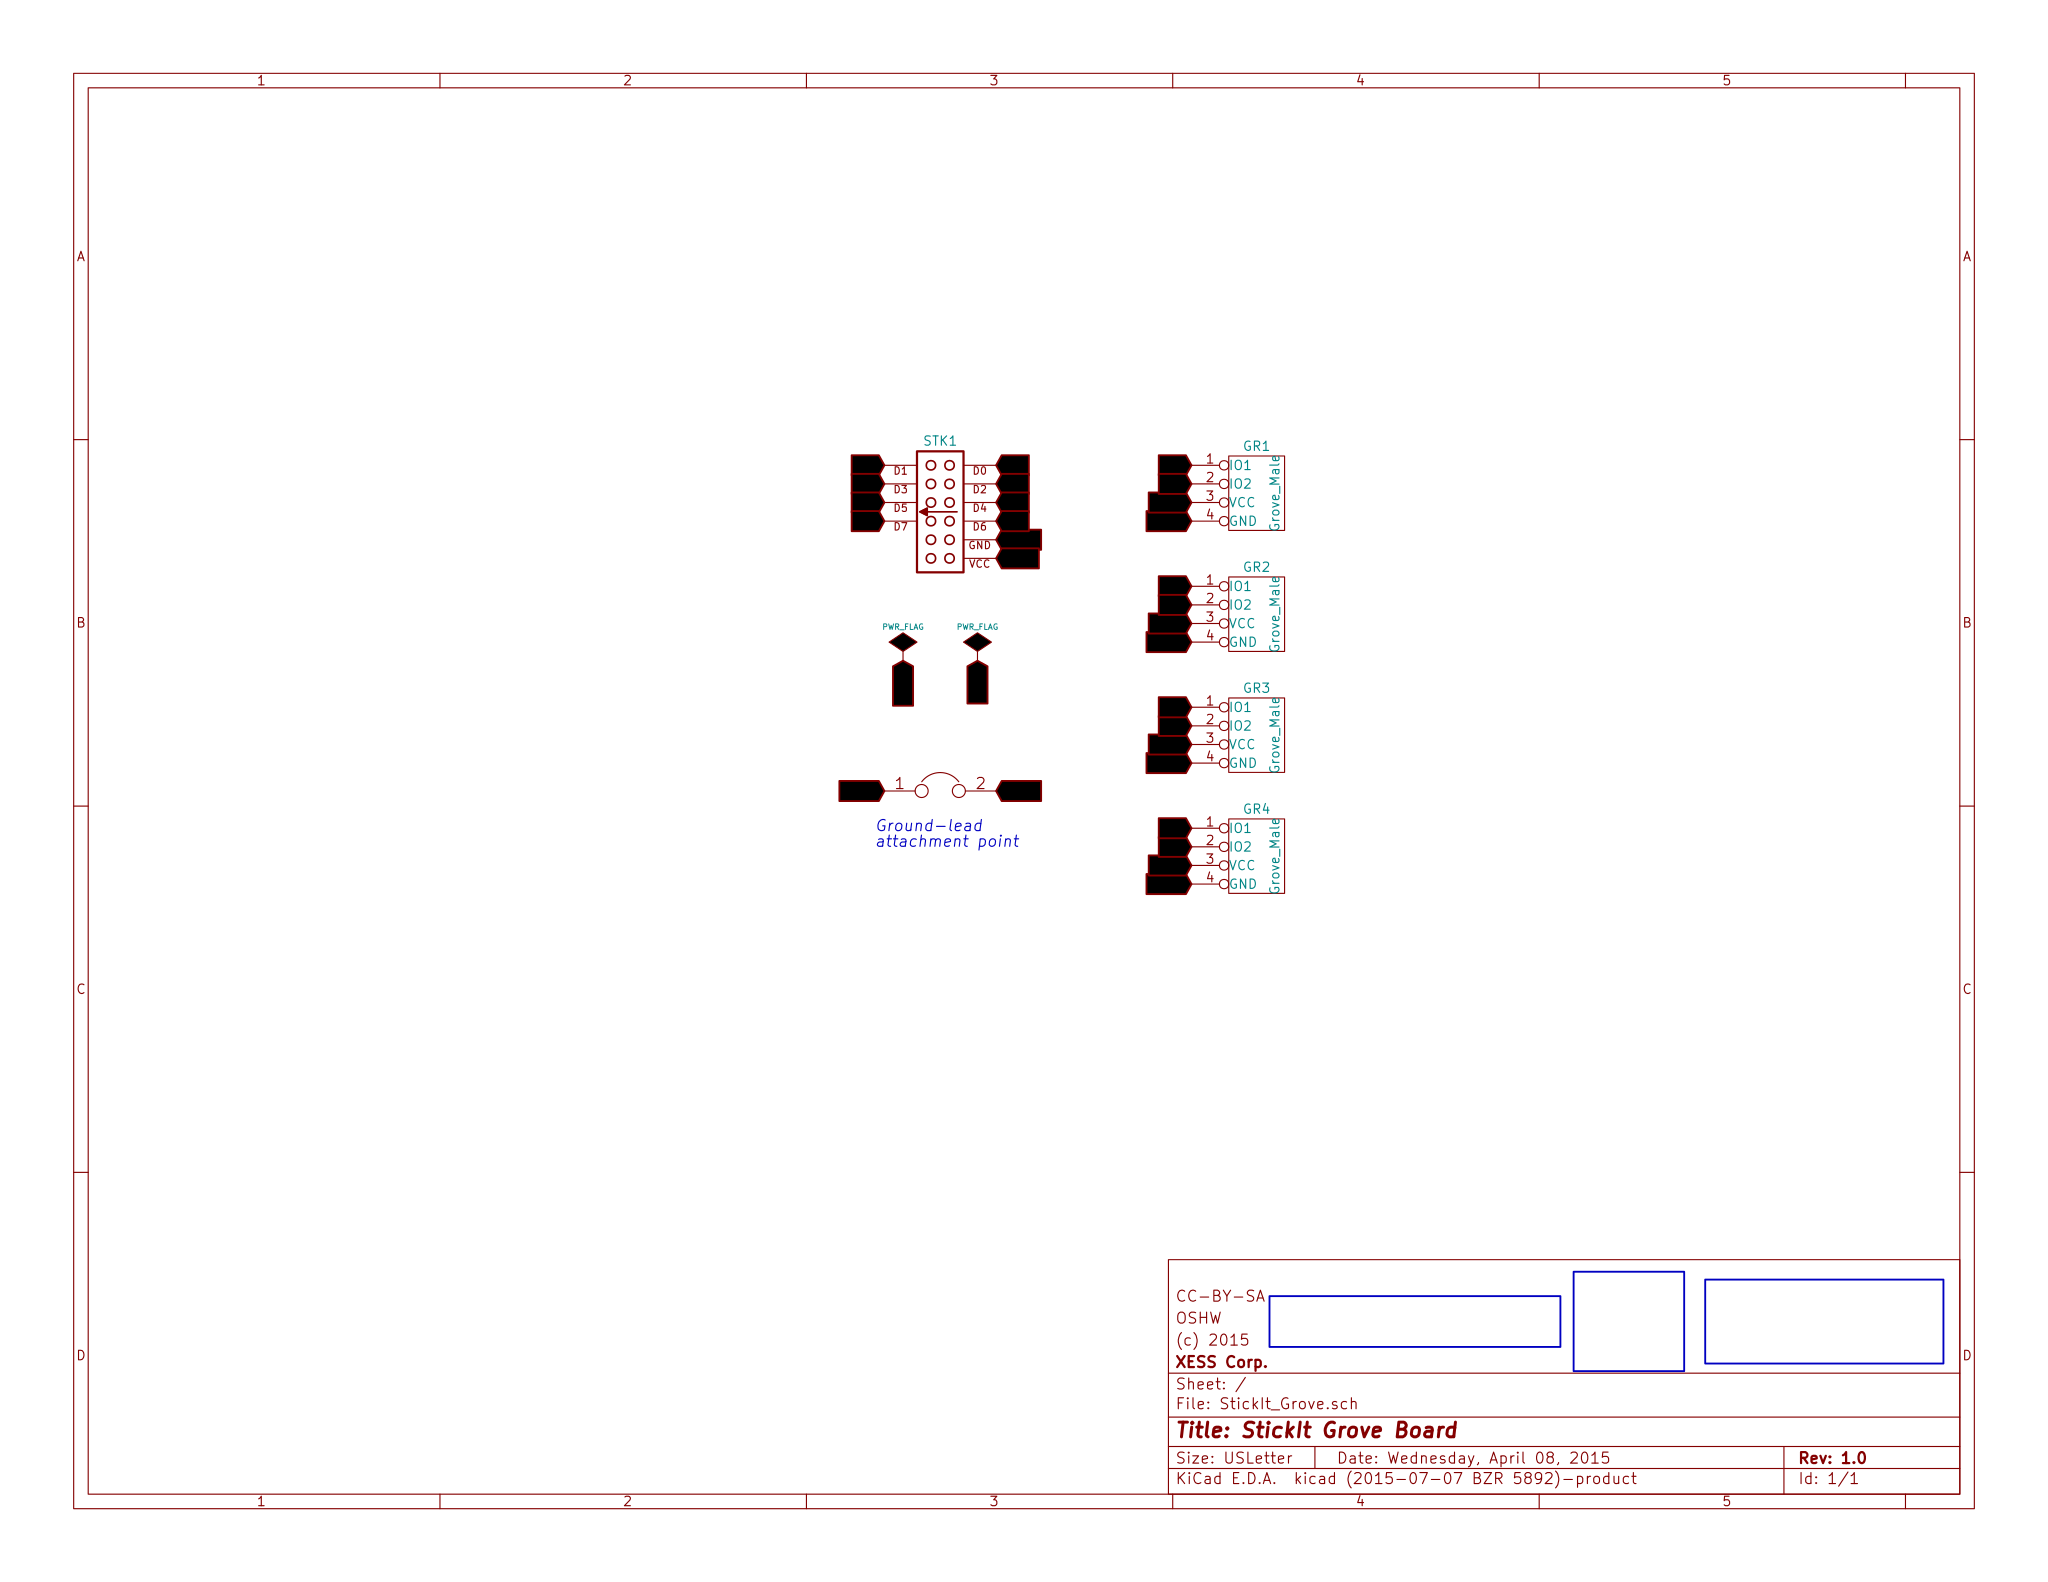
\includegraphics[width=\textheight, angle=90]{grove_schematic.png}}


\end{document}
